% Created 2021-03-19 Fri 13:50
% Intended LaTeX compiler: pdflatex
\documentclass[smaller]{beamer}
\PassOptionsToPackage{colorlinks}{hyperref}
\usepackage[utf8]{inputenc}
\usepackage[T1]{fontenc}
\usepackage{graphicx}
\usepackage{grffile}
\usepackage{longtable}
\usepackage{wrapfig}
\usepackage{rotating}
\usepackage[normalem]{ulem}
\usepackage{amsmath}
\usepackage{textcomp}
\usepackage{amssymb}
\usepackage{capt-of}
\usepackage{hyperref}
\usepackage{blindtext}
\newcommand\mydots{\ifmmode\ldots\else\makebox[1em][c]{.\hfil.\hfil.}\thinspace\fi}
\renewcommand<>{\texttt}[1]{\only#2{\textttorig{#1}}}
\usetheme{sussex}
\author{P. Lasorak}
\date{\today}
\title{Examples}
\begin{document}

\maketitle
\begin{frame}{Outline}
\tableofcontents
\end{frame}

\section{Introduction}
\label{sec:intro}
\begin{frame}[label={sec:intro}]{Introduction}
\begin{itemize}
  \item Welcome to the sussex Beamer template!
  \item Playing with Beamer is a excellent way to procrastinate.
  \item To compile this pdf: \begin{semiverbatim}pdflatex example.tex\end{semiverbatim}
\end{itemize}
\end{frame}

\section{Theme}
\label{sec:theme}
\begin{frame}[label={sec:theme}]{Theme}
\begin{itemize}
  \item Add \begin{semiverbatim} \\usetheme\{sussex\} \end{semiverbatim} to use the theme.
  \item \begin{semiverbatim} \\usetheme[nova]\{sussex\} \end{semiverbatim} or dune should be available to toggle between the themes soon.
\end{itemize}
\end{frame}

\section{Structure}
\label{sec:strucutre}
\begin{frame}[label={sec:structure}]{Structure}
\begin{itemize}
  \item \begin{semiverbatim}\\section\{Structure\}\end{semiverbatim} are going to appear in the table of content (TOC).
  \item Same for \begin{semiverbatim}\\subsection\{First point\}\end{semiverbatim}
  \item \begin{semiverbatim}\\begin\{frame\}\{Slide Title\}\end{semiverbatim} are going to appear at the top of your Slides.
  \item And don't forget to \begin{semiverbatim}\\end\{frame\}\end{semiverbatim} after your slide!
  \item \begin{semiverbatim}
\\begin\{itemize\}\newline
\\item Bullety bullet point.\newline
\\end\{itemize\}\newline
\end{semiverbatim}
\end{itemize}
\end{frame}

\section{Link}
\label{sec:link}
\begin{frame}[label={sec:link}]{Link}
\begin{itemize}
  \item This is an example of a link \href{https://news.fnal.gov/2018/07/dune-collaboration-completes-interim-design-report-for-gigantic-particle-detectors/}{the IDR}.
  \item Page 1 is a pretty picture of ProtoDUNE.
\end{itemize}
\end{frame}

\section{Code}
\label{sec:code}
\begin{frame}[label={sec:code}]{Code}
\begin{itemize}
\item Wait, I also want to include code!
\begin{itemize}
\item \begin{semiverbatim}const sim::Particle* part = bt->HitToParticle(hit); \end{semiverbatim}
\end{itemize}
\end{itemize}
\end{frame}


\section{Images}
\label{sec:images}
\begin{frame}[label={sec:images}]{Images}
\begin{semiverbatim}
\\center\\includegraphics[height=0.7\\textheight, page=4]\newline
\{backtracker.pdf\}
\end{semiverbatim}
\center\includegraphics[height=0.7\textheight, page=4]{backtracker.pdf}
\end{frame}

\section{Long Text}
\label{sec:longtext}
\begin{frame}[label={sec:longtext}]{Long Text}
\blindtext
\end{frame}


\section{Conclusion}
\label{sec:conclusion}
\begin{frame}[label={sec:conclusion}]{Conclusion}
\begin{itemize}
\item Make your changes here: \href{https://cdcvs.fnal.gov/redmine/projects/dunetpc/repository/revisions/develop/show/dune}{dunetpc repo}
\end{itemize}
\end{frame}
\end{document}